% ta med damping på DP-delle

\documentclass[aspectratio=169,xcolor=dvipsnames]{beamer}
%\usetheme{SimplePlus}

\usepackage{hyperref}
\usepackage{graphicx} % Allows including images
\usepackage{booktabs} % Allows the use of \toprule, \midrule and \bottomrule in tables

%----------------------------------------------------------------------------------------
%	TITLE PAGE
%----------------------------------------------------------------------------------------

\title[PLS]{Grunnleggende PLS for 3AUA} % The short title appears at the bottom of every slide, the full title is only on the title page
%\subtitle{Subtitle}

\author[Fred-Olav] {Fred-Olav Mosdal}

\institute[Gand VGS] % Your institution as it will appear on the bottom of every slide, may be shorthand to save space
{
    Gand VGS \\
    VG3 Automasjon }
\date{\today} % Date, can be changed to a custom date


%----------------------------------------------------------------------------------------
%	PRESENTATION SLIDES
%----------------------------------------------------------------------------------------

\begin{document}
\begin{frame}
\titlepage
\end{frame}



\begin{frame}
	\frametitle{Styringssystemers tre deler}
	\begin{columns}
		\begin{column}{0.5\textwidth}
	\begin{itemize}
		\item Inngangsenheter
		\item styreenheter 
		\item utgangsenheter
	\end{itemize}
		\end{column}
		\begin{column}{0.5\textwidth}
	$$\includegraphics[width=1\textwidth]{../output/noGPLimages/pls01.png}$$
		\end{column}
	\end{columns}
\end{frame}


\begin{frame}
	\frametitle{PLS-ens opprinnelse}
	\begin{columns}
		\begin{column}{0.5\textwidth}
			Ble lansert som erstatning for relestyringer\\
			Opprinnelsen sees fremdeles i det mest vanlige programeringsspråket for PLS-er Ladder Logic Diagram
		\end{column}
		\begin{column}{0.5\textwidth}
	$$\includegraphics[width=1\textwidth]{../output/noGPLimages/Modicon 084.jpg}$$
			\url{https://www.engineering.com/programmable-logic-controllers-the-evolution-of-a-disruptive-technology/}
		\end{column}
	\end{columns}
\end{frame}


\begin{frame}
	\frametitle{Eksempler på PLS-er}
$$\includegraphics[width=1\textwidth]{plc_001.eps}$$
\end{frame}

\begin{frame}
	\frametitle{Eksempler på PLS-er}
$$\includegraphics[width=0.8\textwidth]{plc_002.eps}$$
\end{frame}

\begin{frame}
	\frametitle{Eksempler på PLS-er}
$$\includegraphics[width=0.9\textwidth]{plc_017.eps}$$
\end{frame}
\begin{frame}
	\frametitle{Eksempler på PLS-er}
$$\includegraphics[width=0.8\textwidth]{plc_018.eps}$$
\end{frame}
\begin{frame}
	\frametitle{Eksempler på PLS-er}
$$\includegraphics[width=0.7\textwidth]{plc_003.eps}$$
\end{frame}
\begin{frame}
	\frametitle{Eksempler på PLS-er}
$$\includegraphics[width=0.9\textwidth]{plc_004.eps}$$
\end{frame}
\begin{frame}
	\frametitle{Eksempler på PLS-er}
$$\includegraphics[width=0.5\textwidth]{plc_005.eps}$$
\end{frame}
\begin{frame}
	\frametitle{Eksempler på PLS-er}
$$\includegraphics[width=0.8\textwidth]{plc_007.eps}$$
\end{frame}
\begin{frame}
	\frametitle{Eksempler på PLS-er}
$$\includegraphics[width=0.8\textwidth]{plc_006.eps}$$
\end{frame}
\begin{frame}
	\frametitle{Inngangs- og utgangs tilkoblinger (IO-er)  }
	\framesubtitle{Tilgang til den virkelige verden}			
$$\includegraphics[width=0.8\textwidth]{plc_075.eps}$$
\end{frame}
\begin{frame}
	\frametitle{Inngangs- og utgangs tilkoblinger (IO-er)  }
	\framesubtitle{Tilgang til den virkelige verden}			
$$\includegraphics[width=0.6\textwidth]{plc_008.eps}$$
\end{frame}

\begin{frame}
	\frametitle{Digitale IO-er}
	\framesubtitle{Digital inngang}			
$$\includegraphics[width=0.9\textwidth]{plc_073.eps}$$
\end{frame}

\begin{frame}
	\frametitle{Digitale IO-er}
	\framesubtitle{Digital utgang}			
$$\includegraphics[width=0.9\textwidth]{plc_074.eps}$$
\end{frame}
\begin{frame}
	\frametitle{Sinking og Soursing}
	\begin{columns}
		\begin{column}{0.5\textwidth}
		\begin{itemize}
			\item Inn- eller utgang som er sinking tar imot strøm 
			\item Inn- eller utgang som er soursing gir ut strøm 
		\end{itemize}	
		\end{column}
		\begin{column}{0.5\textwidth}

$$\includegraphics[width=0.9\textwidth]{plc_009.eps}$$
		\end{column}
	\end{columns}
\end{frame}


\begin{frame}
	\frametitle{Sinking og Soursing}
	\begin{columns}
		\begin{column}{0.5\textwidth}
			
$$\includegraphics[width=0.9\textwidth]{plc_010.eps}$$
		\end{column}
		\begin{column}{0.5\textwidth}

$$\includegraphics[width=0.9\textwidth]{plc_011.eps}$$
		\end{column}
	\end{columns}
\end{frame}
\begin{frame}
	\frametitle{Sinking og Soursing}
	\begin{columns}
		\begin{column}{0.5\textwidth}
			
$$\includegraphics[width=1\textwidth]{plc_012_1.eps}$$
		\end{column}
		\begin{column}{0.5\textwidth}

$$\includegraphics[width=1\textwidth]{plc_012_2.eps}$$
		\end{column}
	\end{columns}
\end{frame}


\begin{frame}
	\frametitle{Analoge IO-er}
	Hvilke typer analoge IO-er har Wago\\
	sjekk \url{www.wago.no}
\end{frame}

\begin{frame}
	\frametitle{Strømforsyningsenhet}
	\begin{columns}
		\begin{column}{0.5\textwidth}
			\begin{itemize}
				\item 24VDC eller 230VAC er vanlig
				\item Viktig å skille PLS forsyning fra IO-forsyning slik at feil ute i anlgget ikke gjøre at PLS mister strømforsyning. 
			\end{itemize}

			
		\end{column}

	\end{columns}
\end{frame}

\begin{frame}
	\frametitle{Overføringskabler}
	\begin{columns}
		\begin{column}{0.5\textwidth}
			\begin{itemize}
				\item USB-kabel
				\item RS-232(Ofte med overgang fra USB)
				\item RS-485(Ofte med overgang fra USB)
				\item Ethernet (TCP/IP)
			\end{itemize}

			
		\end{column}

		\begin{column}{0.5\textwidth}
	$$\includegraphics[width=1\textwidth]{../output/noGPLimages/pls02.png}$$
		\end{column}
	\end{columns}
\end{frame}

\begin{frame}
	\frametitle{Inngangs og utgangsenheter}
	\begin{columns}
		\begin{column}{0.5\textwidth}
			Inngangs- og utgangsenheter i en PLS kalles for IO-er. Det kan være:
			\begin{itemize}
				\item Digitale IO-er. DI for innganger og DO for utganger
				\item Analoge IO-er AI for innganger og AO for utgangere
				\item Moduler for å avlese resolvere og enkodere. 
				\item Kommunikasjonsmoduler
			\end{itemize}


			
		\end{column}

		\begin{column}{0.5\textwidth}
%	$$\includegraphics[width=1\textwidth]{../output/noGPLimages/pls03.png}$$
		\end{column}
	\end{columns}
\end{frame}
\begin{frame}
	\frametitle{DO med rele}
	\begin{columns}
		\begin{column}{0.5\textwidth}
			Rele utganger :
			\begin{itemize}
				\item kan være potensialfrie
				\item Kan bryte forholdsvis store strømmer (6-10A)
				\item Kan brukes på AC og DC
			\end{itemize}

			
		\end{column}

		\begin{column}{0.5\textwidth}
	$$\includegraphics[width=1\textwidth]{../output/noGPLimages/pls03.png}$$
		\end{column}
	\end{columns}
\end{frame}

\begin{frame}
	\frametitle{DO med transistor (Transistorutgang}
	\begin{columns}
		\begin{column}{0.5\textwidth}
			Transistorutganger:
			\begin{itemize}
				\item bryter mindre strømmer (0.5 og 1 A er vanlig)
				\item bryter raskere en rele utganger
				\item Finnes i NPN eller PNP utgaver
				\item NPN kalles også low side switching
				\item PNP kalles også high side switching
				\item Kan brukes på DC
			\end{itemize}

			
		\end{column}

		\begin{column}{0.5\textwidth}
	$$\includegraphics[width=1\textwidth]{../output/noGPLimages/pls04.png}$$
		\end{column}
	\end{columns}
\end{frame}

\begin{frame}
	\frametitle{DO med triac}
	\begin{columns}
		\begin{column}{0.5\textwidth}
			\begin{itemize}
				\item Kan bryte mindre AC strømmer en releer
				\item Tåler flere bryte sykluser
			\end{itemize}

			
		\end{column}

		\begin{column}{0.5\textwidth}
	$$\includegraphics[width=0.8\textwidth]{../output/noGPLimages/pls05.png}$$
		\end{column}
	\end{columns}
\end{frame}

\begin{frame}
	\frametitle{Galvaniske skiller}
	\begin{columns}
		\begin{column}{0.5\textwidth}
			\begin{itemize}
				\item Isolerer PLS fra spenninger i felt. 
			\end{itemize}

			
		\end{column}

		\begin{column}{0.5\textwidth}
	$$\includegraphics[width=1\textwidth]{../output/noGPLimages/pls06.png}$$
		\end{column}
	\end{columns}
\end{frame}


\begin{frame}
	\frametitle{Analoge IO-er}
	\begin{columns}
		\begin{column}{0.5\textwidth}
			Analoge innganger (AI)
			\begin{itemize}
				\item 1-5 V
				\item 0-10 V
				\item 2-10 V
				\item 4-20 mA
				\item 0-20 mA
				\item RTD ($\Omega$)
				\item termoelement mV
			\end{itemize}

			
		\end{column}

		\begin{column}{0.5\textwidth}
			\href{https://www.contec.com/support/basic-knowledge/daq-control/analog-io/}{link}
			%	$$\includegraphics[width=1\textwidth]{../output/noGPLimages/pls06.png}$$
		\end{column}
	\end{columns}
\end{frame}

\begin{frame}
	\frametitle{Kompakte og  modulære PLS-er}
	\begin{columns}
		\begin{column}{0.5\textwidth}
			\begin{itemize}
				\item item
			\end{itemize}

			
		\end{column}

		\begin{column}{0.5\textwidth}
	$$\includegraphics[width=1\textwidth]{../output/noGPLimages/pls07.png}$$
		\end{column}
	\end{columns}
\end{frame}

\begin{frame}
	\frametitle{Blokkskjematisk oppbygging av PLS fra inngang til utgang}
	$$\includegraphics[width=1\textwidth]{../output/noGPLimages/pls08.png}$$
\end{frame}

\begin{frame}
	\frametitle{Oppbyggning av Module PLS}
	\begin{columns}
		\begin{column}{0.5\textwidth}
			\begin{itemize}
				\item item
			\end{itemize}

			
		\end{column}

		\begin{column}{0.5\textwidth}
	$$\includegraphics[width=1\textwidth]{../output/noGPLimages/pls09.png}$$
		\end{column}
	\end{columns}
\end{frame}

\begin{frame}
	\frametitle{Elektronisk skjema over Siemens DO rele modul}
	$$\includegraphics[width=1\textwidth]{../output/noGPLimages/pls10.png}$$
\end{frame}
\begin{frame}
	\frametitle{Datakommunikasjon}
Med datakommunikasjon menes utvekslig av data som datamaskiner behandler. 
\end{frame}




\begin{frame}
	\frametitle{Data og dataoverføring}
	\begin{columns}
		\begin{column}{0.5\textwidth}
I PLS systemer er ofte måledata som skal overføres. Det overføres da som et binærtall og konverteres til et annet tallsystem i PLS-en. 

			
		\end{column}

		\begin{column}{0.5\textwidth}
	$$\includegraphics[width=1\textwidth]{../output/noGPLimages/kap5x01}$$
		\end{column}
	\end{columns}
\end{frame}

\begin{frame}
	\frametitle{OSI-modellen}
	\begin{columns}
		\begin{column}{0.5\textwidth}

			\begin{itemize}
				\item      
			\end{itemize}

			
		\end{column}

		\begin{column}{0.5\textwidth}
	$$\includegraphics[width=1\textwidth]{../output/noGPLimages/kap5x02}$$
		\end{column}
	\end{columns}
\end{frame}
\begin{frame}
	\frametitle{Ethernet Type II Rammes}
	\begin{columns}
		\begin{column}{0.5\textwidth}

			\begin{itemize}
				\item      
			\end{itemize}

			
		\end{column}

		\begin{column}{0.5\textwidth}
	$$\includegraphics[width=1\textwidth]{../output/noGPLimages/kap5x03}$$
		\end{column}
	\end{columns}
\end{frame}
\begin{frame}
	\frametitle{Dataoverføringsmodus}
	\begin{columns}
		\begin{column}{0.5\textwidth}

Det er ofte nyttig å snakke om hvilke veier dataoverføringen går. Da snakker vi om simplex, halv duplex og duplex.

			
		\end{column}

		\begin{column}{0.5\textwidth}
	$$\includegraphics[width=1\textwidth]{../output/noGPLimages/kap5x04}$$
		\end{column}
	\end{columns}
\end{frame}
\begin{frame}
	\frametitle{Dataprotokoller}

For at 0 og 1 ere skal gi mening mellom senser og mottaker. Må de benytte en avtale om på hvilken måte dataene kommer. Dette kalles en protokoll. 
	
\end{frame}
\begin{frame}
	\frametitle{Dataoverføringsmetoder}
	\begin{itemize}
		\item Asynkron seriell dataoverføring
		\item Synkron seriell dataoverføring
		\item Parellell dataoverføring
	\end{itemize}
\end{frame}

\begin{frame}
	\frametitle{Asynkron seriel dataoverføring}
	\begin{columns}
		\begin{column}{0.5\textwidth}

			\begin{itemize}
				\item Bruker start og stopp bit
				\item kan bruke paritetsbit. 
				\item Veldig vanlig måte og overføre data på. 
			\end{itemize}

			
		\end{column}

		\begin{column}{0.5\textwidth}
	$$\includegraphics[width=1\textwidth]{../output/noGPLimages/kap5x08}$$
	$$\includegraphics[width=1\textwidth]{../output/noGPLimages/kap5x09}$$
		\end{column}
	\end{columns}
\end{frame}
\begin{frame}
	\frametitle{OSI-modellen}
	\begin{columns}
		\begin{column}{0.5\textwidth}

			\begin{itemize}
				\item 
			\end{itemize}

			
		\end{column}

		\begin{column}{0.5\textwidth}
	$$\includegraphics[width=1\textwidth]{../output/noGPLimages/kap5x21}$$
		\end{column}
	\end{columns}
\end{frame}
\begin{frame}
	\frametitle{Signalmodulering}
	\begin{columns}
		\begin{column}{0.5\textwidth}

			\begin{itemize}
				\item AM - Amplitudemodulering
				\item FM - Frekvensmodulering
			\end{itemize}

			
		\end{column}

		\begin{column}{0.5\textwidth}
	$$\includegraphics[width=1\textwidth]{../output/noGPLimages/kap5x22}$$
		\end{column}
	\end{columns}
\end{frame}
\begin{frame}
	\frametitle{Amplitudemodulering av dititalt signal}
	\begin{columns}
		\begin{column}{0.5\textwidth}

			\begin{itemize}
				\item      
			\end{itemize}

			
		\end{column}

		\begin{column}{0.5\textwidth}
	$$\includegraphics[width=1\textwidth]{../output/noGPLimages/kap5x23}$$
		\end{column}
	\end{columns}
\end{frame}
\begin{frame}
	\frametitle{Frekvensmodulering av dititalt signal}
	\begin{columns}
		\begin{column}{0.5\textwidth}

			\begin{itemize}
				\item      
			\end{itemize}

			
		\end{column}

		\begin{column}{0.5\textwidth}
	$$\includegraphics[width=1\textwidth]{../output/noGPLimages/kap5x24}$$
		\end{column}
	\end{columns}
\end{frame}
\begin{frame}
	\frametitle{Fasemodulering (PM) av dititalt signal}
	\begin{columns}
		\begin{column}{0.5\textwidth}

			\begin{itemize}
				\item      
			\end{itemize}

			
		\end{column}

		\begin{column}{0.5\textwidth}
	$$\includegraphics[width=1\textwidth]{../output/noGPLimages/kap5x25}$$
		\end{column}
	\end{columns}
\end{frame}
\begin{frame}
	\frametitle{Smarte instrumenter og HART}
	\begin{columns}
		\begin{column}{0.5\textwidth}

			\begin{itemize}
				\item      
			\end{itemize}

			
		\end{column}

		\begin{column}{0.5\textwidth}
	$$\includegraphics[width=1\textwidth]{../output/noGPLimages/kap5x27}$$
		\end{column}
	\end{columns}
\end{frame}
\begin{frame}
	\frametitle{HART-protokoll}
	\begin{columns}
		\begin{column}{0.5\textwidth}

			\begin{itemize}
				\item      
			\end{itemize}

			
		\end{column}

		\begin{column}{0.5\textwidth}
	$$\includegraphics[width=1\textwidth]{../output/noGPLimages/kap5x28}$$
		\end{column}
	\end{columns}
\end{frame}
\begin{frame}
	\frametitle{Håndterminaler og vedlikehold}
	\begin{columns}
		\begin{column}{0.5\textwidth}

	$$\includegraphics[width=1\textwidth]{../output/noGPLimages/kap5x30}$$

			
		\end{column}

		\begin{column}{0.5\textwidth}
	$$\includegraphics[width=1\textwidth]{../output/noGPLimages/kap5x29}$$
		\end{column}
	\end{columns}
\end{frame}

\begin{frame}
	\frametitle{Kommunikasjonsmoduler}
	\begin{columns}
		\begin{column}{0.5\textwidth}
			\begin{itemize}
				\item item
			\end{itemize}

			
		\end{column}

		\begin{column}{0.5\textwidth}
	$$\includegraphics[width=1\textwidth]{../output/noGPLimages/pls11.png}$$
		\end{column}
	\end{columns}
\end{frame}
\begin{frame}
	\frametitle{Modbus}
	\begin{columns}
		\begin{column}{0.5\textwidth}

			\begin{itemize}
				\item utgitt av modicon i 1979, elste kommnunikasjonsprotokoll innenfor automatisering
				\item er mye utbredt
				\item punkt til punkt og multidrop
				\item Modbus ASCII, Modbus Plus, Modbus RTU og Modubs TCP
			\end{itemize}

			
		\end{column}

		\begin{column}{0.5\textwidth}
	$$\includegraphics[width=1\textwidth]{../output/noGPLimages/kap5x79}$$
		\end{column}
	\end{columns}
\end{frame}
\begin{frame}
	\frametitle{Modbus dataoverføring med og uten feil}
	$$\includegraphics[width=1\textwidth]{../output/noGPLimages/kap5x80}$$
\end{frame}
\begin{frame}
	\frametitle{Modbus funksjonskoder}

	\url{https://ozeki.hu/p_5873-modbus-function-codes.html}

\end{frame}

\begin{frame}
	\frametitle{Logiske funksjoner}
	\begin{columns}
		\begin{column}{0.5\textwidth}
			\begin{itemize}
				\item item
			\end{itemize}

			
		\end{column}

		\begin{column}{0.5\textwidth}
	$$\includegraphics[width=1\textwidth]{../output/noGPLimages/pls12.png}$$
		\end{column}
	\end{columns}
\end{frame}

\begin{frame}
	\frametitle{Logiske funksjoner}
	\begin{columns}
		\begin{column}{0.5\textwidth}
			\begin{itemize}
				\item item
			\end{itemize}

			
		\end{column}

		\begin{column}{0.5\textwidth}
	$$\includegraphics[width=1\textwidth]{../output/noGPLimages/pls13.png}$$
		\end{column}
	\end{columns}
\end{frame}

\begin{frame}
	\frametitle{Data typer}
	\begin{columns}
		\begin{column}{0.5\textwidth}
			\begin{itemize}
				\item item
			\end{itemize}

			
		\end{column}

		\begin{column}{0.5\textwidth}
	$$\includegraphics[width=1\textwidth]{../output/noGPLimages/pls14.png}$$
		\end{column}
	\end{columns}
\end{frame}

\begin{frame}
	\frametitle{Subnett maske og CIDR}% Dette kap stammer fra kollega Ingve Bjørnå
	Hvordan IP-nettverk deles opp

	\begin{columns}
		\begin{column}{0.5\textwidth}
			\begin{itemize}
				\item item
			\end{itemize}

			
		\end{column}

		\begin{column}{0.5\textwidth}
	$$\includegraphics[width=1\textwidth]{../output/noGPLimages/pls15.png}$$
		\end{column}
	\end{columns}
\end{frame}
\begin{frame}
	\frametitle{IP-adressen (IPv4)}
			\begin{itemize}
				\item Alt som vil koble seg til et nettverk trenger en IP-adresse
				\item Består av 32 bit delt opp i 4 med punktum mellom.
				\item $2^{32}$ forskjellige unike IP-adresser (4 294 967 296)
				\item Skrives vanligvis i 10-tall systemet f.eks. slik: 192.168.1.100
				\item I binærtall vil den samme adressen se slik ut:
				\item 1100 0000 . 1010 1000 . 0000 0001 . 0110 0100 (Ikke like enkelt)
			\end{itemize}

			
\end{frame}



\begin{frame}
	\frametitle{Binær og 10 tall systemet}

			\begin{itemize}
				\item En bit er enten 0 eller 1
				\item 8 bit er en byte og en byte er 8 bit
				\item IP-adressen består av 4 byte som er 4 x 8 bit (32 bit)
				\item Det minste en byte kan være er 0000 0000 = 0
				\item Det største en byte kan være er 1111 1111 = 255
				\item En byte kan ha 256 forskjellige verdier, 0 - 255
			\end{itemize}
\end{frame}
\begin{frame}
	\frametitle{En byte er alltid 8 bit}
			\begin{itemize}
				\item Dette gjelder selv om vi ikke bruker alle 8 bit-ene
				\item Tallet 12 i titallsystemet er 1100 i binærtall. 
				\item Hvis 12 er en del av en byte så skrives den slik: 0000 1100
				\item Hvis vi ikke tar med nullene foran blir det feil.
				\item 192.168.1.100
				\item 1100 0000 . 1010 1000 . 0000 0001 . 0110 0100
				\item 1100 0000 . 1010 1000 . 1 . 110 0100 = 192.168.288 (Feil)
			\end{itemize}
\end{frame}
\begin{frame}
	\frametitle{Subnett maske (Nettverksmaske)}

			\begin{itemize}
				\item Deler opp en IP-adresse i Nettverks-ID og Verts-ID (Host-ID)
				\item Nettverks-ID er første del av IP-adressen
				\item Verts-ID er resten av IP-adressen
				\item Kan deles opp på forskjellige plasser ut fra behov
				\item Mange Pcer på samme nett krever at Nettverks-ID får mindre plass og Vets-ID får større plass
				\item Typisk ser en nettverksmaske slik ut: 255.255.255.0


			\end{itemize}
\end{frame}
\begin{frame}
	\frametitle{Nettverksmaske: 255.255.255.0}

			\begin{itemize}

				\item 1Hvis vi skriver dette i binærtall blir det slik:
				\item 11111 1111 . 1111 1111 . 1111 1111 . 0000 0000
				\item 1Den delen hvor nettverksmasken viser enere er Nettverks-ID
				\item 1Delen hvor nettverksmasken viser nullere er Verts-ID (Host ID)
				\item 1Dette betyr at vi kan ha nesten 256 unike Vets-IDer med samme Nettverks-ID. (Nesten fordi noen er satt av til noe annet)
				\item 1Hvis vi trenger flere kan vi f.eks. si at nettverksmasken er slik:
				\item 1255.255.0.0
				\item 1Ca. hvor mange unike Verts-Ider kan vi ha da?

			\end{itemize}
\end{frame}
\begin{frame}
	\frametitle{Nettverksmaske: 255.255.0.0}

			\begin{itemize}
				\item 1111 1111 . 1111 1111 . 0000 0000 . 0000 0000
				\item Nå har vi 256 * 256 forskjellige adresser å bruke til verts-ID
				\item Det er 65 536 forskjellige unike adresser
				\item Kanskje noe overkill om man bare trenger litt mer enn 256…
				\item Det er faktisk mulig å sette skillet inni en av bytene slik:
				\item 1111 1111 . 1111 1111 . 1111 | 0000 . 0000 0000	
					
			\end{itemize}
\end{frame}
\begin{frame}
	\frametitle{Hva blir nettverksmasken?\\1111 1111 . 1111 1111 . 1111 | 0000 . 0000 0000 }

			\begin{itemize}
				\item De to første bytene er bare enere, så de blir 255
				\item Den siste er bare nullere så den blir 0
				\item Da står vi igjen med : 255. 255. ? . 0\\
\begin{center}
\begin{tabular}{ c c c c c c c c}
128 & 64 	& 32 	& 16 	& 8  	& 4	& 2	&  1\\
1 & 1 	& 1 	& 1 	& 0  	& 0	& 0	&  0\\
\end{tabular}
\end{center}
				\item 128 + 64 + 32 + 16 = 240
				\item Nettverksmasken blir 255.255.240.0
				

			\end{itemize}
\end{frame}
\begin{frame}
	\frametitle{Hva blir nettverksmasken?\\ 1111 1111 . 1111 1111 . 1111 1111 . 1 | 000 0000 }


\begin{center}
\begin{tabular}{ c c c c c c c c}
128 & 64 	& 32 	& 16 	& 8  	& 4	& 2	&  1\\
 &  	&  	&  	&   	& 	& 	&  \\
\end{tabular}
\end{center}
\end{frame}
\begin{frame}
	\frametitle{192.168.1.100}

			\begin{itemize}
				\item Hjemme er du på en PC som har denne adressen
				\item Du vet også at nettverksmasken er 255.255.255.0
				\item Hva er nettverks ID?
				\item 192.168.1.0
				\item Hva er Verts-ID?
				\item 100
				\item Hvilke IPer inngår i nettverksmasken?
				\item 192.168.1.1 - 192.168.1.254    (192.168.1.0 - 192.168.1.255)
				\item Den første og den siste kan man ikke bruke!!! De er avholdt til å være Nettverks-ID og kringkasting (Broadcast) Mer om dette en annen gang.

			\end{itemize}
\end{frame}
\begin{frame}
	\frametitle{CIDR-notasjon}

			\begin{itemize}
				\item En annen (enklere?) måte å skrive nettverksmaske på.
				\item Fra forrige side hadde vi følgende info:
				\item Ip-adresse: 192.168.1.100
				\item Nettverksmaske: 255.255.255.0
				\item I CIDR-notasjon skrives det slik:
				\item 192.168.1.100/24
				\item Nå vet jeg alt jeg trenger å vite, men hvordan?
			\end{itemize}
\end{frame}
\begin{frame}
	\frametitle{192.168.1.100/24}

			\begin{itemize}
				\item IP adressen er: 192.168.1.100
				\item /24 betyr at de første 24 bitene i IP-adressen er nettverksmasken
				\item 1111 1111 . 1111 1111 . 1111 1111 . 0000 0000
				\item     8bit  +     8bit  +     8bit  +     0bit = 24bit 
				\item Da vet vi at nettverks-ID = 192.168.1.0
				\item Vi vet også at kringkastings IP er 192.168.1.255 siden vi har 8 bit til verts-ID-adresser
			\end{itemize}
\end{frame}
\begin{frame}
	\frametitle{192.168.1.100/25}

			\begin{itemize}
				\item Hva er nettverksmasken nå?
\begin{center}
\begin{tabular}{ c c c c c c c c}
128 & 64 	& 32 	& 16 	& 8  	& 4	& 2	&  1\\
 &  	&  	&  	&   	& 	& 	&  \\
\end{tabular}
\end{center}
				\item 255.255.255.128
				\item Hvor mange Vertsadresser kan vi ha?
				\item $2^7$ = 128 Vertsadresser (Altså halvparten av 256)
				\item 192.168.1.1 - 192.168.1.127
				\item Hva er nettverks-ID?
				\item NettverksID er den første/laveste IPen i subnettet
				\item Siden VetsID 100 er mindre enn 128 så er NettverksID 192.168.1.0
				\item KringkastingsIPen er 192.168.1.127, som er den høyeste adressen i subnettet.
			\end{itemize}
\end{frame}
\begin{frame}
	\frametitle{192.168.1.200/25}

			\begin{itemize}
				\item Hva er nettverksmasken nå?
\begin{center}
\begin{tabular}{ c c c c c c c c}
128 & 64 	& 32 	& 16 	& 8  	& 4	& 2	&  1\\
 &  	&  	&  	&   	& 	& 	&  \\
\end{tabular}
\end{center}
				\item 255.255.255.128 (Akkurat det samme som sist)
				\item Hvor mange Vertsadresser kan vi ha?
				\item $2^7$ = 128 Vertsadresser (Fortsatt samme som sist) men nå er vi i et annet subnet enn sist, for vi er over halvparten av 256.
				\item Hva er nettverks-ID?
				\item Nå er Verts-ID over 128. Det betyr at Nettverks-ID er  192.168.1.128 og kringkasting er 192.168.1.255
			\end{itemize}
\end{frame}
\begin{frame}
	\frametitle{En annen måte å se ting på}

			\begin{itemize}
				\item Hvis vi ser på 192.168.1.10 /24 så er den siste byten avsatt til verts-IDer
				\item Hvis vi ser på 192.168.1.10 /25 så er bare 7 bit satt av til verts-IDer og en av bitene hører til Nettverks-ID
				\item Et bit kan ha 2 tilstander: 0 og 1. den er 0 når den siste byten er under 128 og 1 når den er 128 og oppover.
				\item 0111 1111 = 127
				\item 1000 0000 = 128 
				\item Hvis IPen slutter på noe over 128 betyr det at du er i den øverste halvdelen, og nettverks-ID er 192.168.1.128
				\item Hvis IPen slutter på noe lavere enn 127 så betyr det at nettverks-ID er 192.168.1.0
				\item Ipen slutta på 10, så derfor er nettverks-ID 192.168.1.0
			\end{itemize}
\end{frame}
\begin{frame}
	\frametitle{Fortsettelse}

	\begin{columns}
		\begin{column}{0.5\textwidth}

			\begin{itemize}
				\item vis vi ser på 192.168.1.10 /26, hvordan skal vi tenke da?
				\item Nå har vi 2 bit som hører til nettverks-ID og 6 som hører til Verts-ID.
				\item 2 bit kan ha 4 tilstander: 00, 01, 10 og 11
				\item Det betyr at IP-adressen er i en av 4 forskjellige subnet
				\item Vi deler inn subnettene slik:
				\item Da ser vi at 192.168.1.10 tilhører det første subnettet
				\item Derfor er nettverks-ID 192.168.1.0
				\item Broadcast er 192.168.1.63 
			\end{itemize}
			
		\end{column}

		\begin{column}{0.5\textwidth}
\begin{tabular}{ c c }
	Område & Tilstander\\
	0-63 & 00 \\
	64-127 & 01 \\
	127-191 & 10 \\
	192-255 & 11 
\end{tabular}
		\end{column}
	\end{columns}
\end{frame}
\begin{frame}
	\frametitle{Hvor fant jeg disse tallene?}

	\begin{columns}
		\begin{column}{0.5\textwidth}

			\begin{itemize}
				\item 63 = \textcolor{red}{00}\textcolor{black}{11 1111}
				\item 64 = \textcolor{red}{01}\textcolor{black}{00 0000}
				\item 127 = \textcolor{red}{01}\textcolor{black}{11 1111}
				\item 128 = \textcolor{red}{10}\textcolor{black}{00 0000}
				\item 191 = \textcolor{red}{10}\textcolor{black}{11 1111}
				\item 192 = \textcolor{red}{11}\textcolor{black}{00 0000}
			\end{itemize}
		\end{column}

		\begin{column}{0.5\textwidth}
\begin{tabular}{ c c }
	Område & Tilstander\\
	0-63 & 00 \\
	64-127 & 01 \\
	127-191 & 10 \\
	192-255 & 11 
\end{tabular}
		\end{column}
	\end{columns}
\end{frame}
\begin{frame}
	\frametitle{Oppgave:}

			\begin{itemize}
				\item 192.168.20.100 /26
				\item Hva er nettverksmasken?
				\item Hvor mange Verts-ID-er kan vi ha på dette subnettet?
				\item Hva er nettverks ID?
				\item Hva er krinkastingsadressen?
			\end{itemize}
\end{frame}
\begin{frame}
	\frametitle{}

			\begin{itemize}
				\item
			\end{itemize}
\end{frame}
\begin{frame}
	\frametitle{}

			\begin{itemize}
				\item
			\end{itemize}
\end{frame}
\begin{frame}
	\frametitle{}

			\begin{itemize}
				\item
			\end{itemize}
\end{frame}
\end{document}
